% !TeX program = xelatex
\documentclass{beamer}
\usepackage{etex} % fixes new-dimension error
%-------------- template --------------------------------------------------
\usetheme{metropolis}
\metroset{block=fill}
%\usetheme{Boadilla}

% Configuring the foot line
\setbeamertemplate{footline}
{
  \leavevmode%
  \hbox{%
  \begin{beamercolorbox}[wd=.4\paperwidth,ht=2.25ex,dp=1ex,center]{author in head/foot}%
    \usebeamerfont{author in head/foot}\insertshortauthor
  \end{beamercolorbox}%
  \begin{beamercolorbox}[wd=.5\paperwidth,ht=2.25ex,dp=1ex,center]{title in head/foot}%
    \usebeamerfont{title in head/foot}\insertsection
  \end{beamercolorbox}%
  \begin{beamercolorbox}[wd=.1\paperwidth,ht=2.25ex,dp=1ex,right]{date in head/foot}%
    \insertframenumber{} / \inserttotalframenumber\hspace*{2ex} 
  \end{beamercolorbox}}%
  \vskip0pt%
}
% No configuration symbols
\makeatother
\setbeamertemplate{navigation symbols}{}

%----------------------------------------------------------------------------
\usepackage{graphicx,amsmath}
\usepackage{stmaryrd} % cf. interleave
\usepackage{booktabs}
\usepackage{amscd}
\usepackage{multicol}
\usepackage[absolute,overlay]{textpos}
\usepackage{alltt}
\usepackage{proof}
%------ using xy ------------------------------------------------------------
\usepackage[all]{xy}
%\def\larrow#1#2#3{\xymatrix{ #3 & #1 \ar[l] _-{#2} }}
\def\larrow#1#2#3{\xymatrix{ #3 & #1 \ar[l] _--{#2} }}
\def\rarrow#1#2#3{\xymatrix{ #1 \ar[r]^-{#2} & #3 }}
\def\arLaw#1#2#3#4#5{
\xymatrix{
        #1      \ar@/^1pc/[rr]^-{#4} &
        #5 &
        #2      \ar@/^1pc/[ll]^-{#3}
}}
\def\arLeq#1#2#3#4{\arLaw{#1}{#2}{#3}{#4}\leq}
%------ using pstricks (rnode etc) ------------------------------------------
\usepackage{pstricks,pst-node,pst-text,pst-3d}
%------ using color ---------------------------------------------------------

\input{macros2}
% No configuration symbols
\makeatother
\setbeamertemplate{navigation symbols}{}
%----------------------------------------------------------------------------
% context
\AtBeginSection[]
{
    \begin{frame}
        \frametitle{Table of Contents}
        \tableofcontents[currentsection]
    \end{frame}
}
\author[Renato Neves]{Renato Neves}

% logos of institutions
\titlegraphic{
  \begin{textblock*}{5cm}(7.8cm,7.45cm)
     
\includegraphics[scale=0.044]{images/uminho.png}\hspace*{.85cm}~%
  \end{textblock*}
  \begin{textblock*}{5cm}(9.8cm,7.45cm)
    
\includegraphics[scale=0.4]{images/haslab.pdf}
  \end{textblock*}
}

% no date
\date{}

\begin{document}

\title{Simply Typed Lambda-Calculus}

\frame[plain]{\titlepage}

\section{The Calculus} 

\begin{frame}{Deductive Reasoning}

  \begin{block}{The essence}
          Knowledge obtained via \alert{assumptions} and
          \alert{logical rules}
  \end{block}

  \bigskip
  Studied since Aristotle  \dots

  \dots\ long before the age of \alert{artificial} computers

  \pause
  \bigskip
  So what does it have to do with programming ?
\end{frame}

\begin{frame}{A Basic Deductive System}
  \begin{minipage}[0.3\textheight]{\textwidth}
  \begin{columns}[c]
  \begin{column}{0.5\textwidth}
          $\typeA,\typeB \dots$ denote \alert{propositions}
          and $\typeOne$ a proposition that always holds   
  \end{column}
  \begin{column}{0.45\textwidth}
        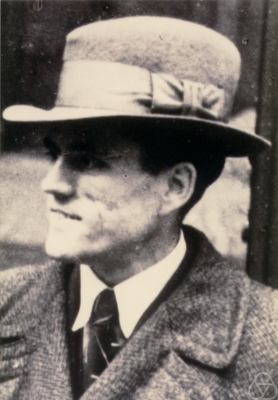
\includegraphics[scale=0.2]{images/gentzen.jpg}
        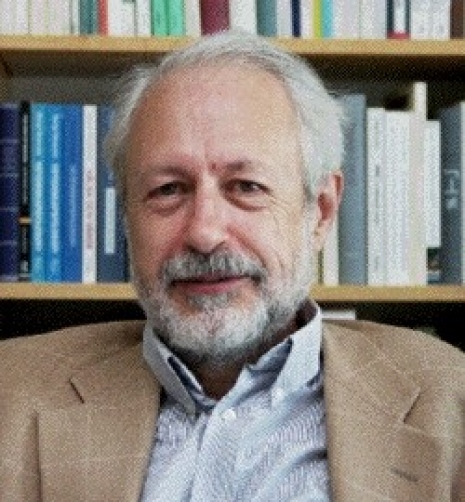
\includegraphics[scale=0.16]{images/prawitz.jpg}
  \end{column}
  \end{columns}
  \end{minipage}

  If $\typeA$ and $\typeB$ are propositions then
  \begin{itemize}
    \item $\typeA \times \typeB$ is a proposition -- 
        conjunction of $\typeA$ and $\typeB$
    \item $\typeA \to \typeB$ is a proposition -- 
            implication of $\typeB$ from $\typeA$
  \end{itemize}
  
\end{frame}

\begin{frame}{A Basic Deductive System}
  
  $\Gamma$ denotes a \alert{list of propositions} (often called context)

  $\Gamma \vljud \typeA$ reads \emph{``if the propositions in $\Gamma$ hold then  $\typeA$ also holds''}

  \small{
  \begin{flalign*}
      \infer[(\rulename{ass})]{\Gamma \vljud \typeA}{\typeA \in \Gamma} \hspace{0.8cm}
      \infer[(\rulename{trv})]{\Gamma \vljud  1}{}  \hspace{0.8cm}
      \infer[(\rulename{\pi_1})]{\Gamma \vljud \typeA}{\Gamma \vljud \typeA \times \typeB} \hspace{0.8cm}
      \infer[(\rulename{\pi_2})]{\Gamma \vljud \typeB}{\Gamma \vljud \typeA \times \typeB}
  \end{flalign*}
  \begin{flalign*}
      \infer[(\rulename{prd})]{\Gamma \vljud \typeA \times \typeB}
      {\Gamma \vljud \typeA \qquad \Gamma \vljud \typeB} \hspace{0.4cm}
      \infer[(\rulename{cry})]{\Gamma \vljud \typeA \to \typeB}{\Gamma, \typeA \vljud  \typeB}
      \hspace{0.4cm}
      \infer[(\rulename{app})]{\Gamma \vljud \typeB}
      {\Gamma \vljud  \typeA \to \typeB \quad
        \Gamma \vljud  \typeA}
  \end{flalign*}
        } 
  
  \bigskip
  \begin{block}{Exercise}
        Show that $\typeA \times \typeB \vdash \typeB \times \typeA$
  \end{block}
 
\end{frame}

\begin{frame}{New Knowledge From Old}
  The rules below are \alert{derivable} from the previous system

  \begin{flalign*}
      \infer[\text{(exchange)}]{\Gamma, \typeB, \typeA,\Delta \vljud \typeC}{
      \Gamma, \typeA, \typeB,\Delta \vljud \typeC}
      \hspace{2cm}
      \infer[\text{(weakening)}]{\Gamma,\typeB \vljud \typeA}{\Gamma \vljud \typeA}
  \end{flalign*}
  \begin{flalign*}
      \infer[\text{(cut elimination)}]{\Gamma\vljud \typeB}{
      \Gamma, \typeA \vljud \typeB \qquad \Gamma \vljud \typeA}
  \end{flalign*}

\end{frame}

\begin{frame}{Exercise}
  Derive the following judgements
  \begin{itemize}
          \item $\typeA \to \typeB,\typeB \to \typeC \vljud \typeA \to \typeC$ 
          \item $\typeA \to \typeB,\typeA \to \typeC \vljud \typeA \to \typeB
                  \times \typeC$
  \end{itemize}        
\end{frame}

\begin{frame}[plain]

        \begin{center}
                Back to programming \dots
        \end{center}
\end{frame}
%
\begin{frame}{The Bare Essentials of Programming}
  %
  The \alert{basic features} of programming
  %
  \begin{itemize}
  \item variables  
  \item function application and creation
  \item pairing \dots
  \end{itemize}
  %
  \bigskip
  %
  %
  \begin{center}
  \fbox{
        Simply-typed $\lambda$-calculus
  }
  \end{center}
  %
  \pause
  The basis of \alert{\texttt{Haskell}}, \texttt{ML},
  \texttt{Eff}, \texttt{F\#}, \texttt{Agda}, \texttt{Elm} and many
  other programming languages
\end{frame}
%
\begin{frame}{Simply-typed Lambda-Calculus}

  Types defined by $\typeA ::= \typeOne \mid \typeA \times \typeA \mid \typeA
  \to \typeA$

  $\Gamma$ now a \alert{non-repetitive} list of typed variables $x_1 : \typeA_1
  \dots x_n : \typeA_n$

  Programs built according to the following \alert{deduction rules}
  \vspace{0.5cm}
  \small{
  \begin{flalign*}
      \infer[(\rulename{ass})]{\Gamma \vljud x : \typeA}{x :
        \typeA \in \Gamma} \hspace{1.2cm}
      \infer[(\rulename{triv})]{\Gamma \vljud \ast : 1}{}  \hspace{1.2cm}
      \infer[(\rulename{\pi_1})]{\Gamma \vljud \pi_1 \, t : \typeA }
      {\Gamma \vljud t: \typeA \times \typeB}
  \end{flalign*}
  \begin{flalign*}
     \infer[(\rulename{prd})]{\Gamma \vljud \langle t,s \rangle :
        \typeA \times \typeB}
      {\Gamma \vljud t: \typeA \qquad \Gamma \vljud s: \typeB} \hspace{1cm}
      \infer[(\rulename{cry})]{\Gamma \vljud \lambda x : \typeA . \, t : \typeA
        \to \typeB}
      {\Gamma, x : \typeA \vljud t : \typeB}
    \end{flalign*}
   \begin{flalign*}
      \infer[(\rulename{app})]{\Gamma \vljud t \, s : \typeB}
      {\Gamma \vljud  t : \typeA \to \typeB \quad
        \Gamma \vljud  s : \typeA}
    \end{flalign*}
   }
\end{frame}
%
\begin{frame}{Examples of $\lambda$-terms}
  \begin{flalign*}
          & x : \typeA \vljud x : \typeA && \text{(identity)}
          \\[15pt]
          & x : \typeA \vljud \langle x, x \rangle : \typeA \times \typeA
          && \text{(duplication)} 
          \\[15pt]
          & x : \alert{\typeA \times \typeB}
          \vljud \langle \pi_2\ x , \pi_1\ x \rangle : \alert{ \typeB \times \typeA }
          && \text{(swap)}
          \\[15pt]
          & f : \alert{\typeA \to \typeB}, g : \alert{\typeB \to \typeC} \vljud
          \lambda x : \typeA . \> g (f \> x) : \alert{\typeA \to \typeC}
          && \text{(composition)}
  \end{flalign*}
\end{frame}
%
\begin{frame}{Exercises}

    Recall the derivations that lead to the judgement
    \[
      \typeA \to \typeB,  \typeA \to \typeC \vljud  \typeA 
      \to \typeB \times \typeC
    \]
    Build the corresponding program

    \bigskip
    Derive as well the judgement 
    \[
        \typeA \to \typeB \vljud  \typeA  \times \typeC
        \to \typeB \times \typeC
    \]
    and subsequently build the corresponding program
\end{frame}
%
\section{Denotational Semantics}
%
\begin{frame}{A Semantics for Simply Typed Lambda-calculus}
  We wish to assign a \alert{mathematical meaning} to $\lambda$-terms
  \begin{flalign*}
    \sem{-} \, : \lambda\text{-terms} \longrightarrow ...
  \end{flalign*}
  so that we can reason about them rigorously, and take advantage
  of known mathematical theories
  \vfill \pause
  
  This is the goal of the next slides. But first \dots
\end{frame}
%
\begin{frame}{Functions: Basic Facts}

  For every set $X$ there exists a `trivial' function
  \begin{flalign*}
    ! : X \longrightarrow \{ \star \} = 1 \hspace{1cm} ! \, (x) = \star
  \end{flalign*}

  We can always pair two functions into
  $f : X \to A$, $g : X \to B$
  \begin{flalign*}
    \langle f,g \rangle: X \to A \times B \hspace{1cm} \langle f,g \rangle (x) = (f \> x, g \> x)
  \end{flalign*}

  There exist projection functions
  \begin{flalign*}
    \pi_1 : X \times Y \to X  \hspace{1cm} \pi_1(x,y) = x \\
    \pi_2 : X \times Y \to Y  \hspace{1cm} \pi_2(x,y) = y
  \end{flalign*}
\end{frame}
%
\begin{frame}{Functions: Basic Facts}

  We can always curry a function $f : X \times Y \to Z$ into
  \begin{flalign*}
    \lambda f : X \to Z^Y \hspace{1cm} \lambda f (x) = (y \mapsto f(x,y))
  \end{flalign*}

  Consider sets $X,Y, Z$. There exists an application function
  \begin{flalign*}
    \mathrm{app} : Z^Y  \times Y \to Z \hspace{1cm}
    \mathrm{app}(f,y) = f \> y
  \end{flalign*}
\end{frame}
%
\begin{frame}{Denotational Semantics}
  Types $\typeA$ interpreted as \alert{sets} $\sem{\typeA}$
  \begin{flalign*}
    \sem{1} & = \{ \star \} \\
    \sem{\typeA \times \typeB} & = \sem{\typeA} \times \sem{\typeB} \\
   \sem{\typeA \to \typeB} & = \sem{\typeB}^{\sem{\typeA}} 
 \end{flalign*}

 Typing contexts $\Gamma$ interpreted as Cartesian products
 \begin{flalign*}
  \sem{\Gamma}\ = \sem{x_1 : \typeA_1, \dots, x_n : \typeA_n}\ =
 \sem{\typeA_1} \times \dots \times \sem{\typeA_n} 
 \end{flalign*}

 Terms $\Gamma \vljud t : \typeA$ interpreted as \alert{functions}
 \begin{flalign*}
   \sem{\Gamma \vljud t : \typeA}\ : \sem{\Gamma}\ \longrightarrow \sem{\typeA}
 \end{flalign*}

\end{frame}
%
\begin{frame}{Denotational Semantics}
 Term $\Gamma \vljud t : \typeA$ interpreted as a function
 \begin{flalign*}
   \sem{\Gamma \vljud t : \typeA}\ : \sem{\Gamma}\ \longrightarrow \sem{\typeA}
 \end{flalign*}
 \vspace{-0.5cm}
 \small{
   \begin{flalign*}
      \infer[]{\sem{\Gamma \vljud x_i : \typeA} = \pi_i}{x_i :
        \typeA \in \Gamma} \hspace{1.2cm}
      \infer[]{\sem{\Gamma \vljud \ast : 1}\ =\ !}{}  \hspace{1.2cm}
      \infer[]{\sem{\Gamma \vljud \pi_1 t : \typeA} = \pi_1 \cdot f }
      {\sem{\Gamma \vljud t : \typeA \times \typeB} = f}
  \end{flalign*}
  \begin{flalign*}
      \infer[]{\sem{\Gamma \vljud \langle t,s \rangle :
        \typeA \times \typeB}\ = \langle f,g \rangle}
    {\sem{\Gamma \vljud t: \typeA}\ = f \qquad \sem{\Gamma \vljud s: \typeB}\ = g}
    \hspace{0.3cm}
     \infer[]{\sem{\Gamma \vljud \lambda x : \typeA . \, t : \typeA
        \to \typeB}\ = \lambda f}
      {\sem{\Gamma, x : \typeA \vljud t : \typeB}\ = f}
    \end{flalign*}
   \begin{flalign*}
      \infer[]{\sem{\Gamma \vljud t \, s : \typeB}\ = \mathrm{app} \cdot \langle f,g \rangle}
      {\sem{\Gamma \vljud  t : \typeA \to \typeB}\ = f \quad
        \sem{\Gamma \vljud  s : \typeA}\ = g}
    \end{flalign*}
}
\end{frame}
%
\newcommand{\pv}[1]{\langle #1 \rangle}
%
\begin{frame}{The Unravelling}
        \begin{align*}
                & \sem{x \vljud \pv{ \pi_2 \, x, \, \pi_1 \, x} } &  = \dots 
                &
                \\
                & \sem{- \vljud \lambda x. \, \pv{ \pi_2 \, x, \, \pi_1 \, x} } & = \dots 
                &
                \\[10pt]
                & \sem{f, g , x \vljud g \, f \, x} & = \dots
                &
                \\
                & \sem{f, g \vljud \lambda x. \, g \, f \, x} & = \dots
                &
                \\[10pt]
                & \sem{f, x \vljud \pv{f \, \pi_1 \, x, \, \pi_2 \, x} \, } & = \dots
                &
                \\
                & \sem{f \vljud \lambda x. \, \pv{f \, \pi_1 \, x, \, \pi_2 \, x} \, } & = \dots
                &
                \\
                & \sem{- \vljud \lambda f. \, \lambda x. \, \pv{f \, \pi_1 \,
                x, \, \pi_2 \, x} \, } & = \dots &
        \end{align*}
        \vfill
        \begin{center}
                (\scriptsize{\textbf{N.B.} all types omitted for simplicity})
        \end{center}
\end{frame}
%
\begin{frame}{More exercises}
  Show that the following equations hold
  \begin{flalign*}
    \sem{x, y \vljud \pi_1 \pv{x,y}}\ & =\
    \sem{x , y \vljud x } \\[5pt]
    \sem{\Gamma \vljud t}\ & =\
    \sem{\Gamma \vljud \langle \pi_1\ t, \pi_2\ t \rangle }
    \\[5pt]
    \sem{ x \vljud (\lambda y. \, \pv{x,y})\>  \> x  }\,
                                    & =\
                                    \sem{ x \vljud \pv{x,x}  }
  \end{flalign*}
\end{frame}
%
\end{document}
